\documentclass[11pt]{article}
\usepackage{graphicx}
\usepackage{hyperref}
%\usepackage{appendix}
\usepackage{amsmath}
\usepackage{amsthm}
\usepackage{amssymb}
\usepackage{float}
\usepackage{commath}
%\usepackage{siunitx}
%\sisetup{detect-all}
\usepackage{listings}
\usepackage{color} %red, green, blue, yellow, cyan, magenta, black, white
\definecolor{mygreen}{RGB}{28,172,0} % color values Red, Green, Blue
\definecolor{mylilas}{RGB}{170,55,241}
\usepackage[a4paper,margin=20mm]{geometry}
\numberwithin{equation}{section}
\setlength{\parskip}{\baselineskip}
\setlength{\parindent}{0pt}
\hypersetup{
    colorlinks=true,
    linkcolor=magenta,
    filecolor=magenta,      
    urlcolor=magenta,
}
\urlstyle{same}
\begin{document}
\title{\textbf{UCL Mechanical Engineering 2020/2021}\\ENGF0004 Coursework 2}
\author{NCWT3}
\maketitle
\section{Question 1}
\subsection{a}
For the line integral to be independent from the path of integration, the following conditions must be fulfilled:
\begin{gather}
    I = \int_A^B \left(\frac{\partial u}{\partial x} \dif x + \frac{\partial u}{\partial y}\dif y\right)\\
    P\left(x, \, y\right) = \frac{\partial u}{\partial x} \textrm{ and } Q\left(x, \, y\right) = \frac{\partial u}{\partial y}\\
    \frac{\partial P\left(x, \, y\right)}{\partial y} = \frac{\partial Q\left(x, \, y\right)}{\partial x}
\end{gather}
Considering the integral:
\begin{gather}
    I = \int_A^B \left[e^{-\alpha xy} \left(\frac{\alpha-2}{x}\right)\dif x - \frac{1}{\alpha y}\left(e^{-\alpha x y}-1\right)\dif y\right]\\
    P\left(x, \, y\right) = e^{-\alpha xy} \left(\frac{\alpha-2}{x}\right) \textrm{ and } Q\left(x, \, y\right) = - \frac{1}{\alpha y}\left(e^{-\alpha x y}-1\right)\\
    \frac{\partial P\left(x, \, y\right)}{\partial y} = -\alpha x \left(\frac{\alpha -2}{x}\right) e^{-\alpha xy} = \left(2\alpha - \alpha^2\right)e^{-\alpha xy}\\
    \frac{\partial Q\left(x, \, y\right)}{\partial x} = -\frac{1}{\alpha y}\left(-\alpha y\right)e^{-\alpha xy} = e^{-\alpha xy}\\
    \therefore 2\alpha e^{-\alpha xy} - \alpha^2 e^{-\alpha xy} = e^{-\alpha xy}\\
    e^{-\alpha xy} \left(\alpha^2 - 2\alpha + 1\right) = 0\\
    e^{-\alpha xy} = 0 \rightarrow \textrm{no solutions}\\
    \left(\alpha - 1\right)^2 = 0\\
    \alpha = 1
\end{gather}
\subsection{b}
Calculating the line integral of \ref{1beq1} from $O\left(0, \, 0\right)$ to $A(1, \, e-1)$ along $y=e^x -1$:
\begin{gather}
    I = \int_O^A \left(ye^{-2x}\right)\left(\dif x + \dif y\right) \label{1beq1}\\
    y = e^x - 1\\
    \dif y = e^x \dif x\\
    I = \int_0^1 \left( \left( e^x-1\right) \left( e^{-2x} \right) + \left( e^x-1\right)\left( e^{-2x}\right)\left( e^x\right)\right)\dif x \\
    = \int_0^1 \left(e^{-x} - e^{-x} - e^{-2x} +1\right)\dif x\\
    = \int_0^1 \left(1-e^{-2x}\right)\dif x \\
    = \left[x + \frac{e^{-2x}}{2}\right]_0^1\\
    = 1 + \frac{e^{-2}}{2} -0-\frac{1}{2}\\
    I = \frac{1}{2}\left(e^{-2}+1\right)
\end{gather}
\subsection{c}
\subsubsection{i}
\begin{gather}
    \underline{F}\left(x, \, y, \, z\right) = \begin{pmatrix}
        \frac{y}{x^2}\\
        \frac{x}{y^2}
    \end{pmatrix}\\
    \nabla \cdot \underline{F} = \begin{pmatrix}
        \frac{\partial}{\partial x}\\
        \frac{\partial}{\partial y}
    \end{pmatrix} \cdot \begin{pmatrix}
        \frac{y}{x^2}\\
        \frac{x}{y^2}
    \end{pmatrix}\\
    = \frac{\partial}{\partial x}\left(\frac{y}{x^2}\right) + \frac{\partial}{\partial y} \left(\frac{x}{y^2}\right)\\
    = -\frac{2y}{x^3}-\frac{2x}{y^3} \\
    = -2\left(\frac{y}{x^3}+\frac{x}{y^3}\right)
\end{gather}
\subsubsection{ii}
\begin{gather}
    I = \int_{1}^{2} \int_{1}^{2} \left(-2\left(\frac{y}{x^3}+\frac{x}{y^3}\right)\right) \dif x \dif y\\
    = \int_{1}^{2} \left[-2\left(\frac{y}{-2x^2} + \frac{x^2}{2y^3}\right)\right]_1^2 \dif y\\
    = \int_{1}^{2} \left[-2\left(-\frac{y}{8} + \frac{2}{y^3}+\frac{y}{2} - \frac{1}{2y^3}\right)\right] \dif y\\
    = \int_{1}^{2} \left(-\frac{3y}{4}-\frac{3}{y^3}\right) \dif y\\
    = \left[-\frac{3y^2}{8}+\frac{3}{2y^2}\right]_1^2\\
    = -\frac{3}{2} + \frac{3}{8} + \frac{3}{8} - \frac{3}{2}\\
    I = -\frac{9}{4}
\end{gather}
\subsection{d}
\subsubsection{i}
\begin{gather}
    I = \int \left(\sin x \cos y \dif y + \cos x \sin y \dif y\right)\\
    y = 0 \hspace{1cm} \dif y = 0\\
    I_{AB} = \int_{x=0}^{\pi} \left(\sin x\right)\dif x = \left[-\cos x\right]_0^{\pi} = 2\\
    x = \pi \hspace{1cm} \dif x = 0\\
    I_{BC} = \int_{y=0}^{\pi} \left(-\sin y\right)\dif y= \left[\cos y\right]_0^{\pi} = -2\\
    \therefore I = I_{AB} + I_{BC} = 2-2 = 0
\end{gather}
\subsubsection{ii}
\begin{gather}
    I = \int \left(\sin x \cos y \dif y + \cos x \sin y \dif y\right)\\
    y = x \hspace{1cm} \dif y = \dif x\\
    I_{AC} = \int_0^{\pi} \left(\sin x \cos x + \sin x \cos x\right) \dif x\\
    = \int_0^{\pi} \left(\sin \left(2x\right)\right)\dif x\\
    I_{AC} = \left[-\frac{1}{2}\cos \left(2x\right)\right]_0^{\pi} = \frac{1}{2} - \frac{1}{2} = 0\\
\end{gather}
\subsection{e}
\subsubsection{i}
\begin{figure}[H]
    \centering
    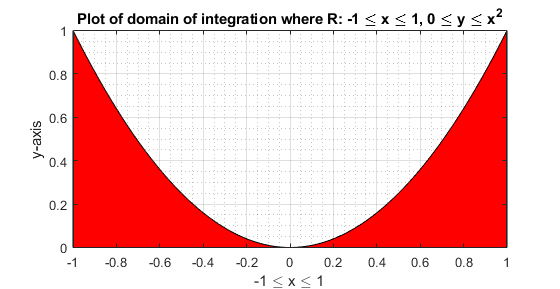
\includegraphics[width = 0.75 \textwidth]{./img/q1ei.png}
    \caption{Domain of integration where $R: \, -1 \leq x \leq 1, \, 0 \leq y \leq x^2$.}
\end{figure}
\lstset{language=Matlab,%
    %basicstyle=\color{red},
    breaklines=true,%
    morekeywords={matlab2tikz},
    keywordstyle=\color{blue},%
    morekeywords=[2]{1}, keywordstyle=[2]{\color{black}},
    identifierstyle=\color{black},%
    stringstyle=\color{mylilas},
    commentstyle=\color{mygreen},%
    showstringspaces=false,%without this there will be a symbol in the places where there is a space
    numbers=left,%
    numberstyle={\tiny \color{black}},% size of the numbers
    numbersep=9pt, % this defines how far the numbers are from the text
    emph=[1]{for,end,break},emphstyle=[1]\color{red}, %some words to emphasise
    %emph=[2]{word1,word2}, emphstyle=[2]{style},    
}
\lstinputlisting{q1ei.m}
\subsubsection{ii}
\subsection{f}
\subsubsection{ii}
\begin{figure}[H]
    \centering
    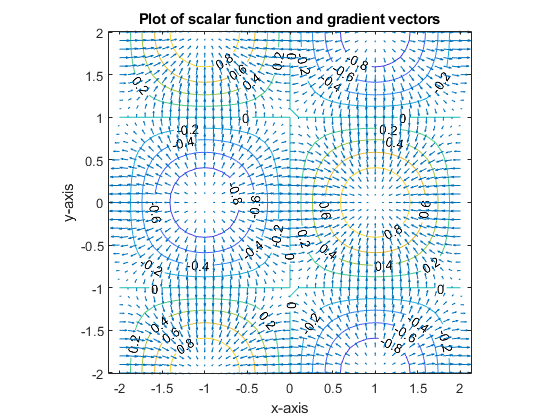
\includegraphics[width = 0.75 \textwidth]{./img/q1fii.png}
    \caption{}
\end{figure}
\lstset{language=Matlab,%
    %basicstyle=\color{red},
    breaklines=true,%
    morekeywords={matlab2tikz},
    keywordstyle=\color{blue},%
    morekeywords=[2]{1}, keywordstyle=[2]{\color{black}},
    identifierstyle=\color{black},%
    stringstyle=\color{mylilas},
    commentstyle=\color{mygreen},%
    showstringspaces=false,%without this there will be a symbol in the places where there is a space
    numbers=left,%
    numberstyle={\tiny \color{black}},% size of the numbers
    numbersep=9pt, % this defines how far the numbers are from the text
    emph=[1]{for,end,break},emphstyle=[1]\color{red}, %some words to emphasise
    %emph=[2]{word1,word2}, emphstyle=[2]{style},    
}
\lstinputlisting{q1fii.m}
\section{Question 2}
\subsection{a}
In our series of equations, there are three unknown internal bar forces $N_{12}$, $N_{23}$, $N_{13}$, and three unknown reaction forces, $R_{2x}$, $R_{2y}$, $R_{3y}$. We also have two unknown angles, $\alpha$ and $\beta$, and the force $F$. Given that there are six unknowns that we would like to find and six equations with those variables, the conditions are fulfilled to solve this using matrices. Our answer would be in terms of the variables $\alpha$, $\beta$ and $F$. Values may be assumed, measured or calculated for these.
\subsection{b}
\begin{gather}
    \begin{bmatrix}
        -\cos \alpha & 0 & \cos \beta & 0 & 0 & 0\\
        -\sin \alpha & 0 & -\sin \beta & 0 & 0 &0\\
        \cos \alpha & 1 & 0 & 1 & 0 & 0\\
        \sin \alpha & 0 & 0& 0 & 1 & 0\\
        0 & -1 & -\cos \beta & 0 & 0 & 0\\
        0 & 0 & \sin \beta & 0 & 0 & 1
    \end{bmatrix} \begin{bmatrix}
        N_{12}\\
        N_{23}\\
        N_{13}\\
        R_{2x}\\
        R_{2y}\\
        R_{3y}        
    \end{bmatrix} = \begin{bmatrix}
        0\\
        F\\
        0\\
        0\\
        0\\
        0\\
    \end{bmatrix}
\end{gather}
\subsection{c}
\lstset{language=Matlab,%
    %basicstyle=\color{red},
    breaklines=true,%
    morekeywords={matlab2tikz},
    keywordstyle=\color{blue},%
    morekeywords=[2]{1}, keywordstyle=[2]{\color{black}},
    identifierstyle=\color{black},%
    stringstyle=\color{mylilas},
    commentstyle=\color{mygreen},%
    showstringspaces=false,%without this there will be a symbol in the places where there is a space
    numbers=left,%
    numberstyle={\tiny \color{black}},% size of the numbers
    numbersep=9pt, % this defines how far the numbers are from the text
    emph=[1]{for,end,break},emphstyle=[1]\color{red}, %some words to emphasise
    %emph=[2]{word1,word2}, emphstyle=[2]{style},    
}
\lstinputlisting{q2c.m}
This returned the following:
\begin{gather}
    \begin{bmatrix}
        N_{12}\\
        N_{23}\\
        N_{13}\\
        R_{2x}\\
        R_{2y}\\
        R_{3y}        
    \end{bmatrix} = \begin{bmatrix}
        -800\\
        480\\
        -600\\
        0\\
        640\\
        360
    \end{bmatrix}
\end{gather}
\subsection{d}
\lstset{language=Matlab,%
    %basicstyle=\color{red},
    breaklines=true,%
    morekeywords={matlab2tikz},
    keywordstyle=\color{blue},%
    morekeywords=[2]{1}, keywordstyle=[2]{\color{black}},
    identifierstyle=\color{black},%
    stringstyle=\color{mylilas},
    commentstyle=\color{mygreen},%
    showstringspaces=false,%without this there will be a symbol in the places where there is a space
    numbers=left,%
    numberstyle={\tiny \color{black}},% size of the numbers
    numbersep=9pt, % this defines how far the numbers are from the text
    emph=[1]{for,end,break},emphstyle=[1]\color{red}, %some words to emphasise
    %emph=[2]{word1,word2}, emphstyle=[2]{style},    
}
\lstinputlisting{q2d.m}
This returned the following:
\begin{gather}
    \begin{bmatrix}
        N_{12}\\
        N_{23}\\
        N_{13}\\
        R_{2x}\\
        R_{2y}\\
        R_{3y}        
    \end{bmatrix} = \begin{bmatrix}
        -800\\
        480\\
        -600\\
        0\\
        640\\
        360
    \end{bmatrix}
\end{gather}
\subsection{e}
Matlab App Developer was utilised to create a user friendly interface for inputting the Force $F$, the lengths of each member (as shown in the diagram) and the coefficient matrix. The code is shown below.
\lstset{language=Matlab,%
    %basicstyle=\color{red},
    breaklines=true,%
    morekeywords={matlab2tikz},
    keywordstyle=\color{blue},%
    morekeywords=[2]{1}, keywordstyle=[2]{\color{black}},
    identifierstyle=\color{black},%
    stringstyle=\color{mylilas},
    commentstyle=\color{mygreen},%
    showstringspaces=false,%without this there will be a symbol in the places where there is a space
    numbers=left,%
    numberstyle={\tiny \color{black}},% size of the numbers
    numbersep=9pt, % this defines how far the numbers are from the text
    emph=[1]{for,end,break},emphstyle=[1]\color{red}, %some words to emphasise
    %emph=[2]{word1,word2}, emphstyle=[2]{style},    
}
\lstinputlisting{q2eApp_exported.m}
\begin{figure}[H]
    \centering
    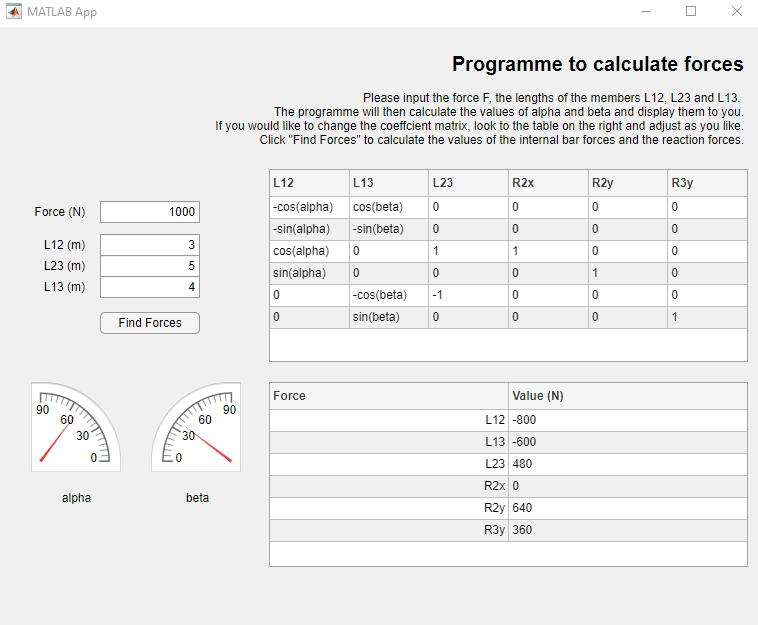
\includegraphics[width = 0.75 \textwidth]{./img/q2e.png}
    \caption{Screenshot from Matlab App, showcasing GUI, input and output parameters.}
\end{figure}
\end{document}